
\documentclass{article}

\usepackage[utf8]{inputenc}
\usepackage{braket}
\usepackage{enumitem}
\usepackage{multirow}
\usepackage{xcolor}
\usepackage[T1]{fontenc}
% \usepackage[french]{babel}
\usepackage{amssymb}
\usepackage{mathtools}
\usepackage{ntheorem}
\usepackage{amsmath}
\usepackage{amssymb}
\usepackage[ a4paper, hmargin={2cm, 2cm}, vmargin={2cm, 2cm}]{geometry}
\usepackage{hyperref}
\usepackage{capt-of}

\usepackage{tikz}
\usetikzlibrary{angles,quotes}

\theoremstyle{plain}
\theorembodyfont{\normalfont}
\theoremseparator{~--}
\newtheorem*{define}{Definition}%[section]
\newtheorem*{ex}{Example}%[section]
\newtheorem*{obs}{Observation}%[section]

\newcommand{\norm}[1]{\left\lVert#1\right\rVert}

\usepackage{hyperref}
\hypersetup{
    colorlinks,
    citecolor=black,
    filecolor=black,
    linkcolor=blue,
    urlcolor=blue
}

\title{TD n$^\circ$1}
\author{Valeran MAYTIE}
\date{}

\begin{document}
  \maketitle

  An isomorphism $f : A \to B$ such that there exists $g: B \to A$ such that $g
  \circ f = Id_A$ and $f \circ g = Id_B$.

  \begin{enumerate}
    \item Show that $g$ is unique
    \item Show that in the following situation

    \begin{center}
      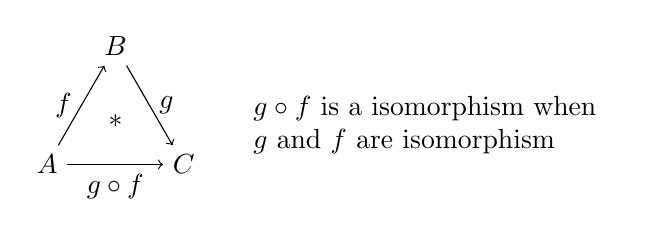
\begin{tikzpicture}
        \node at (0, 0) {*};
        \node (A) at (210:1) {$A$};
        \node (B) at (90 :1) {$B$};
        \node (C) at (330:1) {$C$};

        \draw[->] (A) edge node[left]  {$f$} (B)
                  (B) edge node[right] {$g$} (C)
                  (A) edge node[below] {$g\circ f$} (C);

        \node[text width=4.5cm] at (4, 0)
          {$g \circ f$ is a isomorphism when $g$ and $f$ are isomorphism};
      \end{tikzpicture}
    \end{center}

    \item deduce in $(*)$ that $g$ is an isomorphism when $f$ and $g \circ f$ are
      isomorphism
    \item deduce in $(*)$ that $f$ is an isomorphism when $g$ and $g \circ f$ are
      isomorphism
    \item Suppose that in $A \xrightarrow{f} B \xrightarrow{g} A \xrightarrow{h}
      B$ one has $g \circ f = Id_A$ and $h \circ g = Id_B$ show that $f = h$
      in that case
    \item Characterize the isomorphisms in the category {\bf Set} of sets and
      function. {\bf Top} of topological spaces and continuous functions
  \end{enumerate}

  \newpage
  \underline{\bf Correction} :

  \begin{enumerate}
    \item Let $h : B \to A$ a morphism that $h \circ f = Id_A$ and
      $f \circ h = Id_B $
      \begin{align*}
        h &= h \circ Id_B & \text{By neutrality}\\
          &= h \circ (f \circ g) & \\
          &= (h \circ f) \circ g & \text{By associativity} \\
          &= Id_A \circ g & \\
          &= g & \text{By neutrality}
      \end{align*}

      We can say that $g$ is unique. We will make note $f^{-1}$

    \item We have $f^{-1}$ and $g^{-1}$ the inverse of $f$ and $g$ (they are
      isomorphism)

      We will show that $f^{-1} \circ g^{-1}$ is an inverse of $g \circ f$
      \begin{align*}
        (f^{-1} \circ g^{-1}) \circ (g \circ f) &=
        f^{-1} \circ (g^{-1} \circ g) \circ f & \text{By associativity} \\
        &= f^{-1} \circ f & \\
        &= Id_A &
      \end{align*}

      A similar reasoning can be used to show :$(g \circ f) \circ (f^{-1} \circ
      g^{-1}$

    \item Let $g' = f \circ (g \circ f)^{-1}$
      \begin{align*}
        g \circ g' &= g \circ (f \circ (g \circ f)^{-1}) &
        g' \circ g &= (f \circ (g \circ f)^{-1}) \circ g \\
        &= (g \circ f) \circ (g \circ f)^{-1} &
        &= f \circ (g \circ f)^{-1} \circ g \circ f \circ f^{-1} \\
        &= Id_C &
        &= f \circ (g \circ f)^{-1} \circ (g \circ f) \circ f^{-1} \\
        & &
        &= f \circ f^{-1} \\
        & &
        &= Id_B
      \end{align*}

      $g$ is well an isomorphism.

    \item Roughly the same proof.

    \item We have :
      \begin{align*}
        f &= (h \circ g) \circ f & h \circ g = Id_B \\
          &= h \circ (g \circ f) & \text{By associativity} \\
          &= h & g \circ f = Id_A
      \end{align*}

      This question implies the first question.

    \item Homomorphism (= A map between two structures, that preserves the
      operations of the structures \\
      $f(x \bullet y) = f(x) \bullet f(y)$)
  \end{enumerate}
\end{document}
